\pdfoutput=1
\documentclass[runningheads]{llncs}

\usepackage[T1]{fontenc}
\usepackage{graphicx}
\usepackage{booktabs}
\usepackage{amsmath}
\usepackage{microtype}
% hyperref: llncs ships an outdated compatibility path that breaks against the
% current hyperref (undefined \Hy@pdfmajorversion). The draft builds without it;
% revisit before camera-ready, when Springer supplies its own class bundle.
%\usepackage[hidelinks]{hyperref}

% Anonymised for double-blind review; set to false for the preprint.
\newif\ifanon
\anontrue

\begin{document}

\title{Multi-Card Retrieval: Purpose-Specific Embedding Views for Aspect-Rich Corpora}

\ifanon
  \author{Anonymous}
  \institute{Anonymous}
\else
  \author{Muralidhar Siddavatam\orcidID{0000-0000-0000-0000}}
  \institute{fn7, Hyderabad, India\\ \email{murali@fn7.io}}
\fi

\maketitle

\begin{abstract}
A document that covers several distinct matters is usually indexed as one dense
vector, which averages those matters together. We quantify the resulting loss and
show how to avoid it cheaply. On a controlled corpus in which each document
carries exactly $k$ near-orthogonal aspects, the similarity between an
aspect-directed query and a pooled document vector decays as $k^{-0.32}$ while
the maximum over per-aspect embeddings stays flat, and retrieval quality follows:
at $k=10$, nDCG@10 falls from 0.682 to 0.273 under pooling but holds at 0.672
under per-aspect cards. On the LIMIT capacity benchmark, where single-vector
retrieval is known to fail, the decisive comparison is against chunking rather
than against pooling: splitting the same text into fixed windows lifts nDCG@10 by
0.076, while splitting it into purpose-aligned cards lifts it by 0.674. The
benefit therefore comes from aligning the unit of representation with the unit
the query asks about, not from storing more vectors per document. We report the
storage multiplier each corpus actually incurs, and we release the code, the
seeds, and every per-query score.
\keywords{Dense retrieval \and Multi-vector representations \and Aspect-based
retrieval \and Reproducibility}
\end{abstract}

\section{Introduction}
\label{sec:intro}

% TODO(G4): motivate from the enterprise problem, keep to 1 page in LNCS.
Enterprise corpora are full of documents that are about several things at once.

\paragraph{Contributions.}
\begin{enumerate}
  \item A measurement of aspect dilution on a controlled corpus, giving a fitted
    decay exponent that is milder than the orthogonality argument predicts
    (Section~\ref{sec:dilution}).
  \item Evidence that purpose alignment, not embedding count, drives the benefit,
    via a chunking control on identical source text (Section~\ref{sec:limit}).
  \item An open, seeded, single-command reproduction of every number reported.
\end{enumerate}

\section{Related work}
\label{sec:related}

% TODO(G4): multi-vector retrieval (late interaction); multi-representation
% indexing; embedding capacity limits; diversification; cost-efficient pipelines.
% Every citation must be verified by the citation checker before submission.

\section{Aspect dilution}
\label{sec:dilution}

We first measure the effect in isolation, on a corpus built so that the number of
aspects per document is a controlled variable.

\paragraph{Construction.}
Each document concatenates $k$ passages drawn from $k$ of ten mutually unrelated
topic pools. Every passage realises one \emph{fact}, a (pool, attribute, action)
triple, and a query asks about one fact in wording that shares no template with
the passages. Relevance is therefore defined by the generative process rather
than assumed: every document carrying a passage that realises the queried fact is
relevant, which yields relevance sets of 3.7 documents per query at $k=1$ rising
to 33.3 at $k=10$. Two representations of the same document are compared: one
pooled embedding of the whole text, and $k$ per-aspect embeddings scored by their
maximum. Both are scored at document level. We use 500 documents and 200 queries
per setting, encoder \texttt{all-MiniLM-L6-v2}, seed 13.

\paragraph{Result.}
Table~\ref{tab:dilution} and Figure~\ref{fig:dilution} report the outcome. The
per-aspect representation holds its similarity to relevant documents almost
exactly constant as $k$ grows, from 0.498 at $k=1$ to 0.493 at $k=10$, while the
pooled representation decays monotonically to 0.235. Retrieval follows: the
pooled system loses more than half its nDCG@10 between $k=1$ and $k=2$ and does
not recover, while the card system stays between 0.556 and 0.682 throughout. At
$k=1$ the two systems are identical by construction, and the measurement confirms
it exactly, which is a useful check on the pipeline.

\begin{table}[t]
\caption{Aspect dilution. Deltas are per-query paired differences,
card system minus pooled, with 95\% bootstrap intervals and paired permutation
$p$-values Holm-corrected across all 21 comparisons. Relevance-set sizes grow
with $k$ by construction, so nDCG is comparable down a column and between the two
systems within a row, but not across rows.}
\label{tab:dilution}
\centering
\begin{tabular}{rrrrrl}
\toprule
$k$ & pooled & cards & $\Delta$ & 95\% CI & win/tie/loss \\
\midrule
1  & 0.682 & 0.682 & $+0.000$ & exact tie & 0/200/0 \\
2  & 0.395 & 0.571 & $+0.177$ & $[+0.145, +0.207]$ & 160/0/40 \\
3  & 0.308 & 0.565 & $+0.257$ & $[+0.226, +0.288]$ & 173/1/26 \\
4  & 0.271 & 0.556 & $+0.285$ & $[+0.253, +0.317]$ & 175/0/25 \\
5  & 0.300 & 0.585 & $+0.285$ & $[+0.251, +0.318]$ & 176/2/22 \\
7  & 0.282 & 0.656 & $+0.374$ & $[+0.339, +0.408]$ & 182/0/18 \\
10 & 0.273 & 0.672 & $+0.399$ & $[+0.360, +0.438]$ & 186/1/13 \\
\bottomrule
\end{tabular}
\end{table}

\begin{figure}[t]
\centering
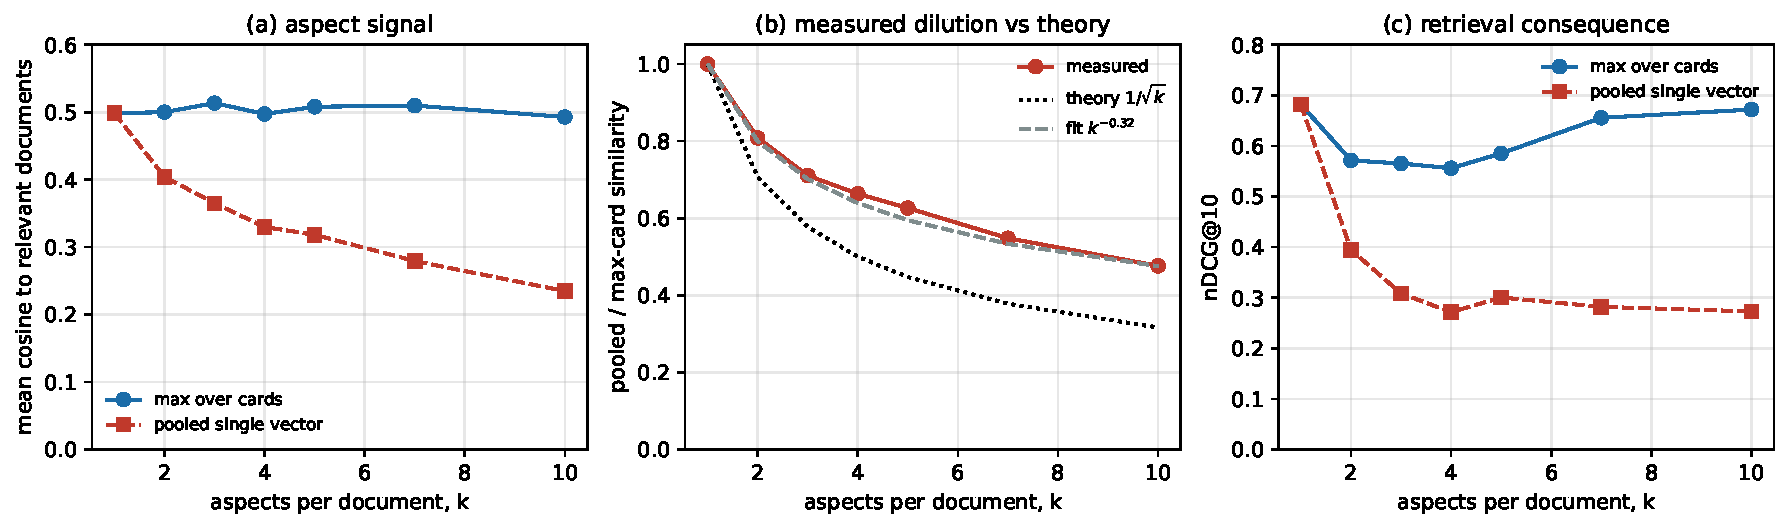
\includegraphics[width=\textwidth]{figures/fig1_dilution.pdf}
\caption{Aspect dilution as a function of $k$. Left: the aspect signal is
preserved by cards and lost by pooling. Centre: measured dilution against the
$1/\sqrt{k}$ prediction and a fitted power law. Right: the retrieval
consequence.}
\label{fig:dilution}
\end{figure}

\paragraph{The theory has the right shape and the wrong magnitude.}
Treating a pooled vector as the normalised mean of $k$ near-orthogonal aspect
vectors predicts that an aspect-directed query's similarity falls as
$1/\sqrt{k}$. The measured ratio of pooled to card similarity instead follows
$k^{-0.32}$, well above the prediction at every $k$. Two properties of real
encoders explain the gap, and both work in the same direction: aspects drawn from
natural language are not orthogonal, since all of the passages share register and
syntax, and encoder similarities are anisotropic, occupying a narrow cone that
compresses differences. We therefore report the orthogonality argument as an
upper bound on dilution rather than as a prediction that the data confirm.


\section{Capacity: does alignment or count explain the gain?}
\label{sec:limit}

The previous section compares cards against a single pooled vector, which leaves
an obvious objection open: cards store more vectors per document, so perhaps
capacity alone explains the gain and any decomposition would do. This section
answers that objection with a control.

\paragraph{Setting.}
LIMIT~\cite{weller2025limit} is constructed to expose the representational
ceiling of single-vector retrieval. Each document names a person and lists the
things they like; each query asks who likes one specific thing. The small variant
has 46 documents, 44.0 attributes each, and 1{,}000 queries, so the task looks
trivial and yet defeats dense retrievers. It also hands us an unambiguous aspect
decomposition, which makes it the sharpest available test of whether alignment
matters. We compare five systems, all scored at document level: BM25; a pooled
dense vector; the same text cut into 30-word windows with 10-word overlap
(186 chunks); the same text cut into per-attribute cards (2{,}024 cards); and
reciprocal rank fusion of the card system with BM25.

\begin{table}[t]
\caption{LIMIT-small. Deltas are against the pooled dense baseline, paired
permutation with Holm correction over 1{,}000 queries. Chunking and carding both
raise the embedding count from one per document to many; only carding recovers
the lost performance.}
\label{tab:limit}
\centering
\begin{tabular}{lrrrrl}
\toprule
system & nDCG@10 & R@2 & R@10 & $\Delta$ vs pooled & $p$ \\
\midrule
BM25                       & 0.997 & 0.991 & 1.000 & $+0.683$ & $<0.001$ \\
dense, pooled              & 0.314 & 0.162 & 0.480 & baseline & \\
dense, 30-word chunks      & 0.390 & 0.225 & 0.549 & $+0.076$ & $<0.001$ \\
dense, per-aspect cards    & 0.988 & 0.965 & 0.997 & $+0.674$ & $<0.001$ \\
cards $\oplus$ BM25 (RRF)  & 0.997 & 0.990 & 1.000 & $+0.683$ & $<0.001$ \\
\bottomrule
\end{tabular}
\end{table}

\paragraph{Alignment, not count.}
Table~\ref{tab:limit} separates the two explanations. Chunking multiplies the
embedding budget and recovers 0.076 nDCG@10. Carding multiplies the same budget
and recovers 0.674, roughly nine times as much, from identical source text under
an identical encoder. The difference between the two is only where the boundaries
fall: a 30-word window spans several attributes and dilutes each of them in the
same way the pooled vector does, whereas a card corresponds to exactly the unit a
query names. Capacity is necessary and not sufficient; the decomposition has to
match the query distribution.

\paragraph{What this result does not show.}
LIMIT supplies a perfect decomposition for free, and its queries are effectively
exact-attribute lookups, which is why BM25 wins outright and the hybrid only
matches it. Real corpora arrive undecomposed, the taxonomy must be designed and
may be misaligned, and the honest reading of this table is as an upper bound on
what alignment can buy rather than as an estimate of what it will buy. We also
note the cost: 44 cards per document here, far above the small constant that the
pattern implies elsewhere, so the storage multiplier is a property of the corpus
and must be reported per corpus rather than assumed.


\section{The first pass: does a cheap gate earn its place?}
\label{sec:gate}

A two-pass design rests on a first pass that is cheap enough to run over
everything and discriminating enough to be worth running. This section tests that
premise, and finds that it holds while two pieces of received practice around it
do not.

\paragraph{Setting.}
On-purpose items are 4,000 messages from a public corporate email corpus;
off-purpose items are 4,000 Usenet posts from unrelated groups. Provenance gives
exact labels at no annotation cost. Three anchor sets describe facets of the
purpose, each item scores the mean of its best few similarities to each set, and
the combination is fitted on one half and reported on the other.

\paragraph{The gate discriminates.}
Held-out ROC-AUC is 0.933 and PR-AUC 0.935. A first pass built from nothing but
embeddings and a handful of anchor phrases separates on-purpose from off-purpose
material well enough to be a filter rather than a sample.

\paragraph{Fitting the weights is worth almost nothing.}
Giving the three anchor sets equal weight yields ROC-AUC 0.931 against 0.933 for
fitted weights. Practitioners tune such weightings at length; on this evidence
the discrimination comes from having several purpose-specific anchor sets at all,
not from how they are mixed.

\begin{table}[t]
\caption{What the gate discards, by recall target. The economic case for a first
pass is proportional to the fraction it removes, and at the high recall such a
filter is supposed to hold, that fraction is modest.}
\label{tab:gate}
\centering
\begin{tabular}{rrrr}
\toprule
recall target & achieved recall & precision & corpus discarded \\
\midrule
0.80 & 0.781 & 0.910 & 57.7\% \\
0.90 & 0.901 & 0.830 & 46.5\% \\
0.95 & 0.954 & 0.710 & 33.7\% \\
0.98 & 0.981 & 0.605 & 20.0\% \\
0.99 & 0.993 & 0.557 & 12.1\% \\
\bottomrule
\end{tabular}
\end{table}

\paragraph{The filter is not where the saving comes from.}
Table~\ref{tab:gate} corrects a common framing. A first pass is usually described
as discarding most of a corpus, but at recall 0.95 it discards about a third, and
at recall 0.99 about an eighth. Gating therefore contributes a linear factor
between one and two, bought directly with recall. The order-of-magnitude saving
in a two-pass design comes from elsewhere: from attaching generative cost to the
number of discovered topics rather than to the number of documents. Attributing
the saving to the filter overstates the filter and understates the substitution.

\paragraph{Caveat.}
Separating corporate email from Usenet is easier than separating on-purpose from
off-purpose material inside one corpus, which is what a deployed gate faces.
These numbers bound discrimination from above; failure here would have been
disqualifying, and success here is necessary rather than sufficient.


\section{Selection: how much diversity, and for whom}
\label{sec:diversity}

The preceding sections concern how a document is represented. This one concerns
what is selected once candidates are retrieved, which is where the study's second
claim lives: that the right amount of diversity depends on who consumes the
results. This section settles the measurable half of that claim, namely what each
policy actually delivers; the consumer half is future work
(Section~\ref{sec:limitations}).

\paragraph{Setting.}
Each of 120 constructed queries is associated with several distinct facts, and
each candidate document realises at most one of them, so the subtopics a
selection covers can be counted exactly rather than inferred. Deriving subtopics
by clustering would have been circular, since one of the policies under test
selects by cluster. Candidates are gated to the upper half by relevance first, as
a first pass would do, and each policy then selects ten items.

\begin{table}[t]
\caption{Selection policies on a constructed coverage task. All coverage gains
over relevance ranking are significant under Holm-corrected paired permutation
tests. Relevance differences are within noise, an artefact of the strong gate
discussed below.}
\label{tab:diversity}
\centering
\begin{tabular}{lrrrr}
\toprule
policy & S-recall & $\alpha$-nDCG & nDCG@10 & answerless rate \\
\midrule
relevance only          & 0.628 & 0.692 & 0.965 & 0.033 \\
MMR, $\lambda=0.7$      & 0.666 & 0.723 & 0.964 & 0.032 \\
MMR, $\lambda=0.3$      & 0.818 & 0.840 & 0.963 & 0.036 \\
DPP                     & \textbf{0.879} & \textbf{0.877} & 0.963 & 0.035 \\
cluster round robin     & 0.666 & 0.724 & 0.967 & 0.028 \\
outlier harvest, 20\%   & 0.716 & 0.734 & 0.966 & 0.031 \\
outlier harvest, 40\%   & 0.772 & 0.775 & 0.967 & 0.028 \\
\bottomrule
\end{tabular}
\end{table}

\paragraph{The operator we proposed is not the best operator.}
Table~\ref{tab:diversity} is not the result we expected. Harvesting the
low-similarity tail of a gated pool does raise coverage substantially, by 0.144
S-recall at a 40 percent quota, but a determinantal point process raises it by
0.251 and maximal marginal relevance at $\lambda=0.3$ by 0.190. We report this
because it sharpens rather than weakens the position we are arguing for. The
claim worth defending is not that a particular diversification operator is best;
it is that the quantity of diversity is a function of the consumer, and that
function applies to whichever operator a system already has. On this evidence the
strongest implementation of the idea is a determinantal point process whose
quality-diversity balance is set per consumer, not the harvest rule.

\paragraph{Under a strong gate, coverage is nearly free.}
No policy paid a measurable relevance penalty, and the answerless rate did not
move. Both follow from gating: when the pool is already bounded for relevance,
spending part of the budget away from its centre costs little and risks little.
This is an argument for the gate rather than evidence that diversity is free, and
we would expect the trade to reappear with a weaker filter or a stricter
relevance criterion.


\section{Limitations}
\label{sec:limitations}

% TODO(G4): expand once the enterprise and encyclopaedic corpora have run.
Three limitations bound what has been shown so far.

First, both results here are on constructed corpora. The synthetic corpus fixes
$k$ by construction, and LIMIT is adversarial by design. Neither tells us what
happens on prose written by people for their own purposes, which is the setting
the pattern is meant for.

Second, the aspect decomposition is given rather than inferred in both cases.
The practical question is whether a taxonomy designed in advance, and applied by
an imperfect extractor, retains a useful share of the benefit.

Third, a single encoder is used throughout. Anisotropy differs between encoders,
and the dilution exponent is likely to move with it.


\section{Reproducibility}
\label{sec:repro}

Every number in this paper is produced by one command per experiment against
committed code and seeds, and every per-query score is released alongside the
aggregates so that the significance tests can be recomputed independently.

Determinism is enforced rather than assumed: two seeded runs must produce
byte-identical per-query output, which is checked in the repository. Reaching
that required accumulating similarity in double precision, because on some
platforms a single-precision matrix product varies by around $10^{-8}$ between
runs with the reduction order, enough to move a recorded value across a rounding
boundary.

Metric implementations are covered by hand-worked golden tests, and the selection
policies by property tests, for example that maximal marginal relevance with
$\lambda = 1$ reduces exactly to relevance ranking and that reciprocal rank fusion
is invariant to the order of its input lists.


\bibliographystyle{splncs04}
\bibliography{refs}

\end{document}
